{\bf
%  \subsubsection{Simulations without a radial}
  \section{Artifical radial density bumps with a radially smooth
    viscosity profile}\label{add_sim}
  In \S\ref{density_bump} we found Rossby vortices became stronger
  as the viscous layer thickness is increased, even though linear growth rates
  were reduced. Here, we present additional simulations to support the 
  hypothesis that this is due to the localised radial structure in the viscosity profile. 

%  For reference we repeated simulation V2 with a floor viscosity
%  $\hat{\nu}_0=10^{-7}$ and all other parameters identical to that in
%  \S\ref{density_bump}. 

  We repeated simulation V2 with the following radially-smooth
  viscosity profile      
  \begin{align}\label{smooth_visc}          
    \hat{\nu}\frac{\rho_i       (R,z)}{B(R)} =
    \hat{\nu}_0\left[1+Q(z/H_0) \right]\frac{\rho_i(r_0,z)}{B(r_0)},
  \end{align}                   
  and $Q$ still given by Eq. \ref{step}. 
  (Recall from Table \ref{artificial_bump} that in
  case V2 the low
  and high viscosity layers occupy $z\in[0,1]H_0$  and
  $z\in[1,2]H_0$ at $R=r_0$, respectively.) We choose a floor viscosity
  of $\hat{\nu}_0=10^{-7}$ to mitigate axisymmetric viscous diffusion of 
  the initial density bump. 

  This simulation is shown as the dotted line in Fig. \ref{appen} 
  in terms of the $m=1$ component of the kinetic energy density. We compare it to an equilvalent run
  employing the radially-structured viscosity profile  of \S\ref{density_bump} (i.e. case V2 
  but with reduced floor viscosity). Although the non-axisymmetric disturbance still grows, it decays 
  monotonically after $|W_1|$ reaches maximum value of $\simeq 0.045$. On the other hand,  
  using the radially-structured viscosity profile (solid line) gives a larger disturbance amplitude at
  the linear stage  ($\max{|W_1|}\simeq0.075$), as well as  the non-linear stage ($|W_1|$ stops decaying for $t\gtrsim110P_0$). 
  The contrast between the two cases shows that the radial structure in the viscosity profile promotes the instability and therefore vortex
  formation and survival. This means that the dominant effect of viscosity on vortex formation via the RWI is its influence on the evolution 
of the axisymmetric component of background disc. 


%  The contrast in Fig. \ref{appen} indicates the viscous evolution of the axisymmetric component of the background 
%  disc

  


 \begin{figure}
  \centering
  \includegraphics[width=\linewidth]{figures/pdisk_kerz_cases_appendix.ps}
  \caption{{\bf Evolution of the $m=1$ component of the kinetic energy density for 
   a disc initialised with a radial density bump in a layered disc. The solid line is a case using 
   the viscosity profile given by Eq. \ref{visc_profile} which accounts for the initial radial density 
   structure, while the dotted line employs the radially-smooth viscosity profile given by Eq. \ref{smooth_visc}.  }
    \label{appen}}
  \end{figure}  
}
